% ****** Start of file apssamp.tex ******
%
%   This file is part of the APS files in the REVTeX 4.2 distribution.
%   Version 4.2a of REVTeX, December 2014
%
%   Copyright (c) 2014 The American Physical Society.
%
%   See the REVTeX 4 README file for restrictions and more information.
%
% TeX'ing this file requires that you have AMS-LaTeX 2.0 installed
% as well as the rest of the prerequisites for REVTeX 4.2
%
% See the REVTeX 4 README file
% It also requires running BibTeX. The commands are as follows:
%
%  1)  latex apssamp.tex
%  2)  bibtex apssamp
%  3)  latex apssamp.tex
%  4)  latex apssamp.tex
%
\documentclass[%
 reprint,
%superscriptaddress,
%groupedaddress,
%unsortedaddress,
%runinaddress,
%frontmatterverbose, 
%preprint,
%preprintnumbers,
%nofootinbib,
%nobibnotes,
%bibnotes,
 amsmath,amssymb,
 aps,
%pra,
%prb,
%rmp,
%prstab,
%prstper,
%floatfix,
]{revtex4-2}

\usepackage{graphicx}% Include figure files
\usepackage{dcolumn}% Align table columns on decimal point
\usepackage{bm}% bold math
\usepackage{url}
\usepackage{algorithm}
\usepackage{algpseudocode}
%\usepackage{hyperref}% add hypertext capabilities
%\usepackage[mathlines]{lineno}% Enable numbering of text and display math
%\linenumbers\relax % Commence numbering lines

%\usepackage[showframe,%Uncomment any one of the following lines to test 
%%scale=0.7, marginratio={1:1, 2:3}, ignoreall,% default settings
%%text={7in,10in},centering,
%%margin=1.5in,
%%total={6.5in,8.75in}, top=1.2in, left=0.9in, includefoot,
%%height=10in,a5paper,hmargin={3cm,0.8in},
%]{geometry}

\begin{document}

\preprint{APS/123-QED}

\title{Constructing a Maximum Tension Coordinate with Neural Networks}
% \thanks{A footnote to the article title}%

\author{Yi Jer Loh}
 \email{yjl34@cam.ac.uk}
\author{Will Handley}
 \email{wh260@cam.ac.uk}
\affiliation{%
 Cavendish Laboratory, 19 J.J. Thomson Avenue, Cambridge CB3 0HE, UK
}%

\date{\today}

\begin{abstract}
An article usually includes an abstract, a concise summary of the work
Lorem ipsum dolor sit amet, consectetur adipiscing elit. Ut ac nisi ex. Sed finibus, sem sit amet tristique vestibulum, elit nibh sagittis eros, et vestibulum odio enim et ante. Interdum et malesuada fames ac ante ipsum primis in faucibus. Donec condimentum libero ligula, nec facilisis diam suscipit eget. Sed accumsan velit nec nisi commodo elementum nec sed ligula. Curabitur rutrum, massa vitae eleifend dictum, enim orci vulputate mi, ac venenatis ante elit quis dolor. Phasellus vitae sapien quis enim convallis bibendum.Mauris nec nulla tellus. Curabitur augue mauris, tristique eget elit vel, ornare congue lectus. Etiam ac vestibulum odio. Nullam blandit ante a turpis maximus tristique. Pellentesque at convallis metus. Etiam elit neque, tincidunt vitae placerat sit amet, rhoncus a justo. 
\end{abstract}

%\keywords{Suggested keywords}%Use showkeys class option if keyword
                              %display desired
\maketitle

%\tableofcontents


\section{Introduction} \label{intro}

With cosmological measurements becoming more precise over recent years, disagreement between different datasets and methods have began to emerge. Observations of parameters surrounding the $\Lambda \textrm{CDM}$ model have yielded discrepancies, or more commonly referred to as \textit{tensions}, of close to $5\sigma$ -- the indication of a significant result in particle physics \cite{Franklin2013}. 

One such tension is the \textit{Hubble tension}. The debate over the Hubble constant's value is one that is hardly new, but in recent years has risen to prominence in cosmology. Disagreement over the Hubble constant began between de Vaucouleurs and Sandage in the 1980s \cite{deVaucouleurs1986, Sandage1975}, and it has now developed into an area of contention between early- and late-universe cosmologists \cite{Planck2020, Abbott2018, Freedman2020, Riess2019, Wong2019}. As it stands, measurements by these two factions are at significant tension of around $5\sigma$ at the most extreme, as shown in Figure \ref{H0_tension}. This has earned the Hubble tension an apt label of a cosmological \textit{crisis}.


\begin{figure}
    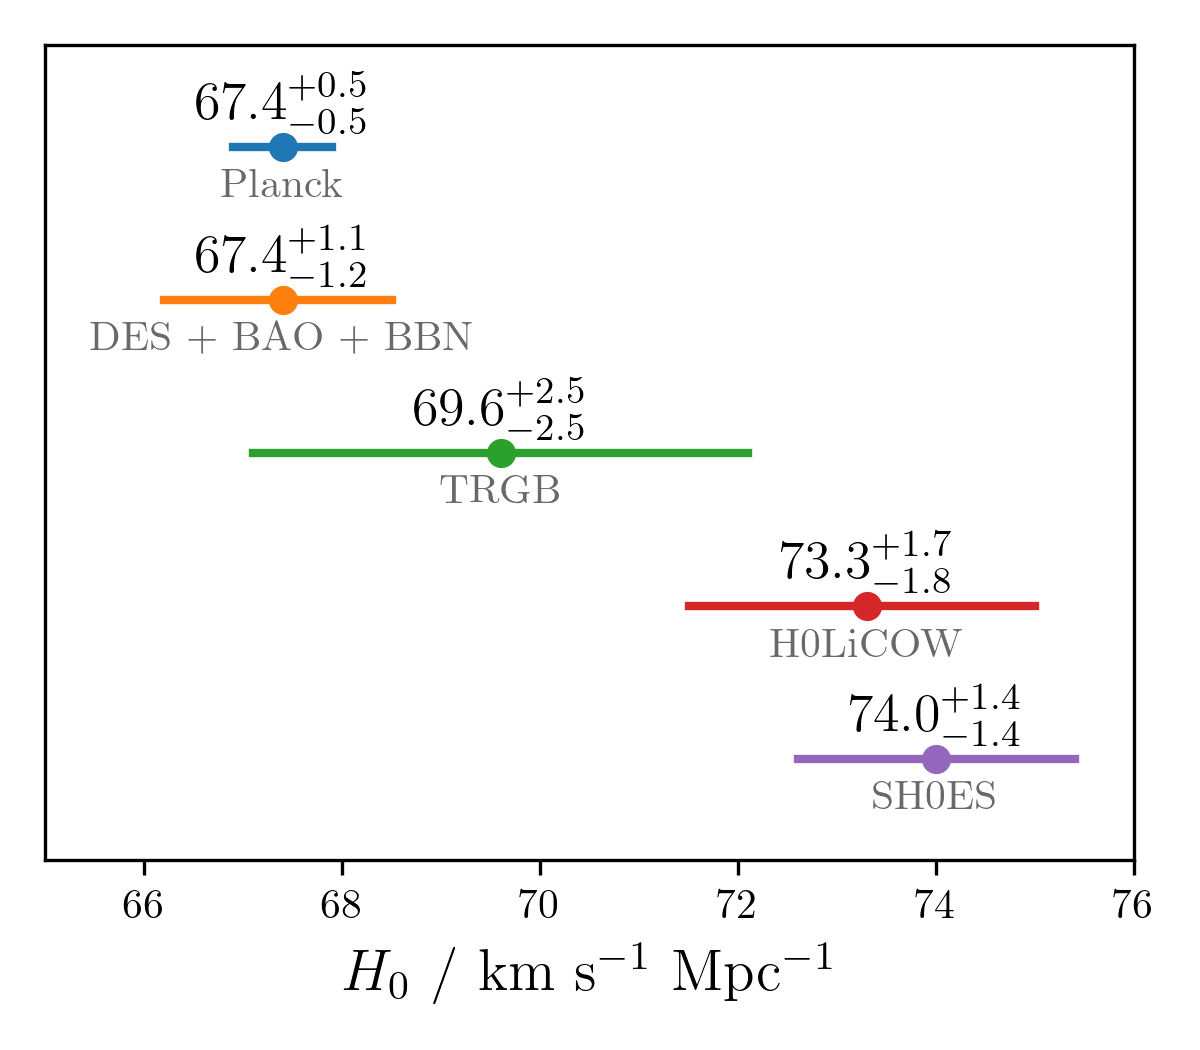
\includegraphics[width=0.8\columnwidth]{../plots/H0 tension.png}
    \centering
    \caption{A compilation of recent measurements of the Hubble constant $H_0$. The top two measurements are from early-universe datasets using $\Lambda$CDM cosmology \cite{Planck2020, Abbott2018}, while the remaining three are from late-universe datasets based off local distance ladder measurements \cite{Freedman2020, Riess2019, Wong2019}. The tension between the \textit{Planck} and SH0ES measurements currently stands at $4.7 \sigma$.}
    \label{H0_tension}
\end{figure}


In addition to the Hubble constant, less severe tensions also exist. Discrepancies of $3\sigma$ have been reported with respect to the matter density $\Omega_m$ and rate of growth of structure $\sigma_8$, between the Cosmic Microwave Background (CMB) data collected by \textit{Planck} and the weak lensing-based Kilo Degree Survey (KiDS) \cite{Heymans2021}. There has also been arguments made for the existence of a "curvature tension", with inconsistencies of $2.5 \sigma$ to $3 \sigma$ between CMB data alluding to a closed curved universe and the tenet of flat curvature in $\Lambda$CDM cosmology \cite{Handley2021Closed}.

These tensions raise questions surrounding the validity of the well-established, well-tested standard cosmological model -- the $\Lambda$CDM. Are these tensions just an artefact of systematic errors from collecting and analysing datasets? Or do these tensions hint at something more fundamental -- perhaps a modification to the standard model, or more excitingly new physics to take the place of the old one?

However, before we make that leap into the realm of new physics, it is essential for us to examine how tension is quantified. With cosmological datasets being multi-dimensional, the problem of quantifying discrepancies is non-trivial. Datasets that appear to be in mild tension, such as the Dark Energy Survey (DES) Y1 and Planck datasets, have been reported to be consistent when using the canonical Bayes factor $R$ \cite{Handley2019}. This is troubling, and is a reflection of the difficulty of the problem. With tensions likely to increase as measurement precision increases, a variety of tension metrics have been proposed in recent literature \cite{Charnock2017} to better understand the problem at hand.

This paper aims to develop on the idea of maximum tension. With cosmological datasets, larger tensions often exist across multiple parameters rather than within each parameter on its own. A good example would be the $3 \sigma$ tension between $\Omega_m$ and $\sigma_8$ -- the tension is obvious in a two-dimensional plot between these two parameters, but is non-existent when the parameters are inspected individually. In a high-dimensional parameter space, it is thus likely that there exists a combination of parameters which exacerbates and maximises tension.

In this paper, we explore how a high-dimensional parameter space can be mapped onto a \textit{tension coordinate} -- a lower-dimensional coordinate which maximises the tension between two datasets. A neural network is used to achieve this mapping, since the non-Gaussian nature of certain cosmological parameters renders an analytical approach challenging. This tension coordinate is then applied to the \textit{Planck} and DES Y1 datasets. Such an approach could allow us to develop a better intuition of the source of tension, and verify the large tensions that currently exist in $H_0$ and the $\Omega_m$-- $\sigma_8$ plane.



\section{Background}

\subsection{Bayesian Statistics}

To describe Bayesian statistics, we use the following notation, with Bayes' theorem written as
\begin{equation}
    P(\theta|D) = \frac{P(D|\theta)P(\theta)}{P(D)} \, \longrightarrow \, \mathcal{P}_D(\theta) = \frac{\mathcal{L}_D(\theta) \pi(\theta)}{\mathcal{Z}_D}.
\end{equation}
The posterior is denoted as $\mathcal{P}_D$, likelihood as $\mathcal{L}_D$, prior as $\pi$, and evidence as $\mathcal{Z}_D$. Note that the subscript here represents the dataset-dependence of these distributions. 

The Bayesian evidence $\mathcal{Z}_D$ is defined as 
\begin{equation}
    \mathcal{Z}_D = \int \mathcal{L}_D \pi \ \rm{d} \theta.
\end{equation}
Also known as the marginal likelihood in statistical literature \cite{Trotta2008}, the evidence is often deemed to be a natural value for model and dataset comparisons within the Bayesian framework. However, the calculation of the evidence is generally computationally inhibitive, as it involves a multi-dimensional integral over the entire parameter space. Fortunately, there are now several tried-and-tested methods that can reliably estimate the evidence, including thermodynamic integration \cite{Lartillot2006} and nested sampling \cite{Skilling2006, Handley2015}.


\subsection{Bayes Factor $R$}

The canonical Bayes factor $R$ \cite{Marshall2006} is our tension metric of choice, and forms the basis of our method in this paper. With two datasets $A$ and $B$, the Bayes factor is expressed as
\begin{equation}
    R = \frac{\mathcal{Z}_{AB}}{\mathcal{Z}_A \mathcal{Z}_B}, \quad \rm{with} \ \mathcal{Z}_{AB} = \int \mathcal{L}_A \mathcal{L}_B \pi \ \rm{d}\theta.
\end{equation}
This factor is defined as the ratio between the probability of $A$ and $B$ describing the same parameter space and the probability of $A$ and $B$ describing separate parameter spaces. A value of $R \gg 1$ thus indicates datasets that are in agreement, and $R \ll 1$ indicates discrepant datasets.

The Bayes factor can be re-expressed as 
\begin{equation}
    R = \int \frac{\mathcal{P}_A \mathcal{P}_B}{\pi} \ \rm{d}\theta.
\end{equation}
This is a more convenient expression to work with, since it does not explicitly call for any evidences. This form of the Bayes factor also makes explicit its prior-dependence, which is arguably a concern \cite{Handley2019}. A broader prior would increase the factor $R$, whilst a narrower prior would reduce $R$ and thus increase tension. Such a dependence means that $R$ is able to hide potential discrepancies with a broad prior. More importantly, consistent datasets with sensible priors \textit{cannot} be reported to be in tension by the Bayes factor, which means that a value of $R$ indicating tension does in fact point to disagreeing datasets, hence low values of $R$ must be taken more seriously. 


\subsection{Tension Coordinate}

Most tension quantification methods, including the Bayes factor, are independent of the choice of parameters and the direction in the parameter space. These methods are not able to describe the spatial structure of the tension, i.e. which parameters contribute most to the tension. As alluded to in the introduction of this paper, it is very probable that there exists a combination of parameters, or more generally a function of the parameter space, which maximises tension between two datasets. The output of such a function is what we call the \textit{tension coordinate}. 

% This coordinate can be expressed as $t = T(\theta)$, where $\theta$ represents the parameter space.

% This idea could be a first step in better understanding the sources of tension between datasets, particularly when one believes there to be more tension than one would expect from a global tension metric.

In this paper, tension is quantified using the Bayes factor $R$. We minimise $R$, calculated in the tension coordinate, to achieve maximum tension. We first demonstrate the tension coordinate for the ideal case of two Gaussian distributions representing two separate datasets. Then, we approach the tension coordinate more practically to tackle non-Gaussian distributions.

\subsubsection{Gaussian example} \label{gaussian_tension}

Let there be two datasets $A$ and $B$ represented by two Gaussian distributions with shared parameters $\theta$. $A$ and $B$ have mean vectors of $\mu_A$ and $\mu_B$, and covariance matrices of $\Sigma_A$ and $\Sigma_B$, respectively. The natural log of the Bayes factor $R$ between these two distributions is written as \cite{Handley2019}
\begin{align}
    \log R &= - \frac{1}{2} (\mu_A - \mu_B)^T (\Sigma_A + \Sigma_B)^{-1} (\mu_A - \mu_B) \\
    &= - \frac{1}{2} \mu^T \Sigma^{-1} \mu.
\end{align}

Define the one-dimensional tension coordinate as a linear combination of the parameters, $t = n^T \theta$. The vector $n$ can be naturally described as the direction of maximum tension. To map the Gaussian distributions onto $t$, we marginalise the distributions onto the hyperplanes perpendicular to $n$. This gives a marginalised Bayes factor of
\begin{align}
    \log R_t &= \frac{1}{2} \big( n^T \mu \big)^T \big( n^T \Sigma n \big)^{-1} \big( n^T \mu \big) \\
    &= \frac{\big( n^T \mu \big)^2}{2 n^T \Sigma n}.
\end{align}

Minimising $\log R_t$ with respect to $n$, which maximises the marginalised tension, gives the direction of maximum tension as
\begin{equation}
    n \propto \Sigma^{-1} \mu = (\Sigma_A + \Sigma_B)^{-1} (\mu_A - \mu_B).
\end{equation}
Substituting this back into the tension coordinate returns
\begin{equation}
    t \propto (\mu_A - \mu_B)^T (\Sigma_A = \Sigma_B)^{-1} \theta
\end{equation}
where $t$ is defined up to a normalisation constant.

\subsubsection{Non-Gaussian case} \label{non_gaussian}

Dataets with non-Gaussian distributions bring more complexity to the tension coordinate. Instead of marginalising the distributions onto hyperplanes, it is more general to marginalise the distributions onto hypersurfaces and define a tension coordinate of $t = T(\theta)$. Note that it is not necessary for $t$ to be one-dimensional, but we restrict ourselves to this in this paper. With this definition of the tension coordinate, the marginalised Bayes factor $R_t$ is expressed as
\begin{equation} \label{margin_R}
    R_t = \int \frac{\mathcal{P}_A^{(T)}(t) \mathcal{P}_B^{(T)}(t)}{\pi^{(T)}(t)} \ \rm{d}t
\end{equation}
where $\mathcal{P}_D^{(T)}(t) = \int \mathcal{P}_D(\theta) \delta(t - T(\theta)) \ \rm{d}\theta$.

In general, we can define a more practical tension coordinate $t = T(\theta; w)$ described by function parameters $w$. To obtain maxiumum tension, the function parameters need to be $w = \arg \min_w R_t$. All of this can be achieved by representing $T$ as a neural network, with $w$ as the weights between nodes and $R_t$ as the loss function for gradient descent. A neural network is an appropriate choice given the \textit{universal approximation theorem}, which states that a multilayer feedforward network is able to approximate any bounded continuous function \cite{Hornik1989}. 


\section{Method}

\subsection{Neural Network and Training}

In this paper, we use a fully-connected neural network with only a single hidden layer with 4096 nodes, as illustrated in Figure \ref{fig:NN}. We find that a single hidden layer is sufficient to fit our maximum tension hypersurfaces around continuous non-Gaussian distributions. The choice of the number of nodes is somewhat arbitrary. Given that this neural network is not used for classification or regression, we do not need to worry about the problem of overfitting our datasets. In fact, one might argue that overfitting might even be a desired effect of the neural network, hence the large number of nodes.

\begin{figure}
    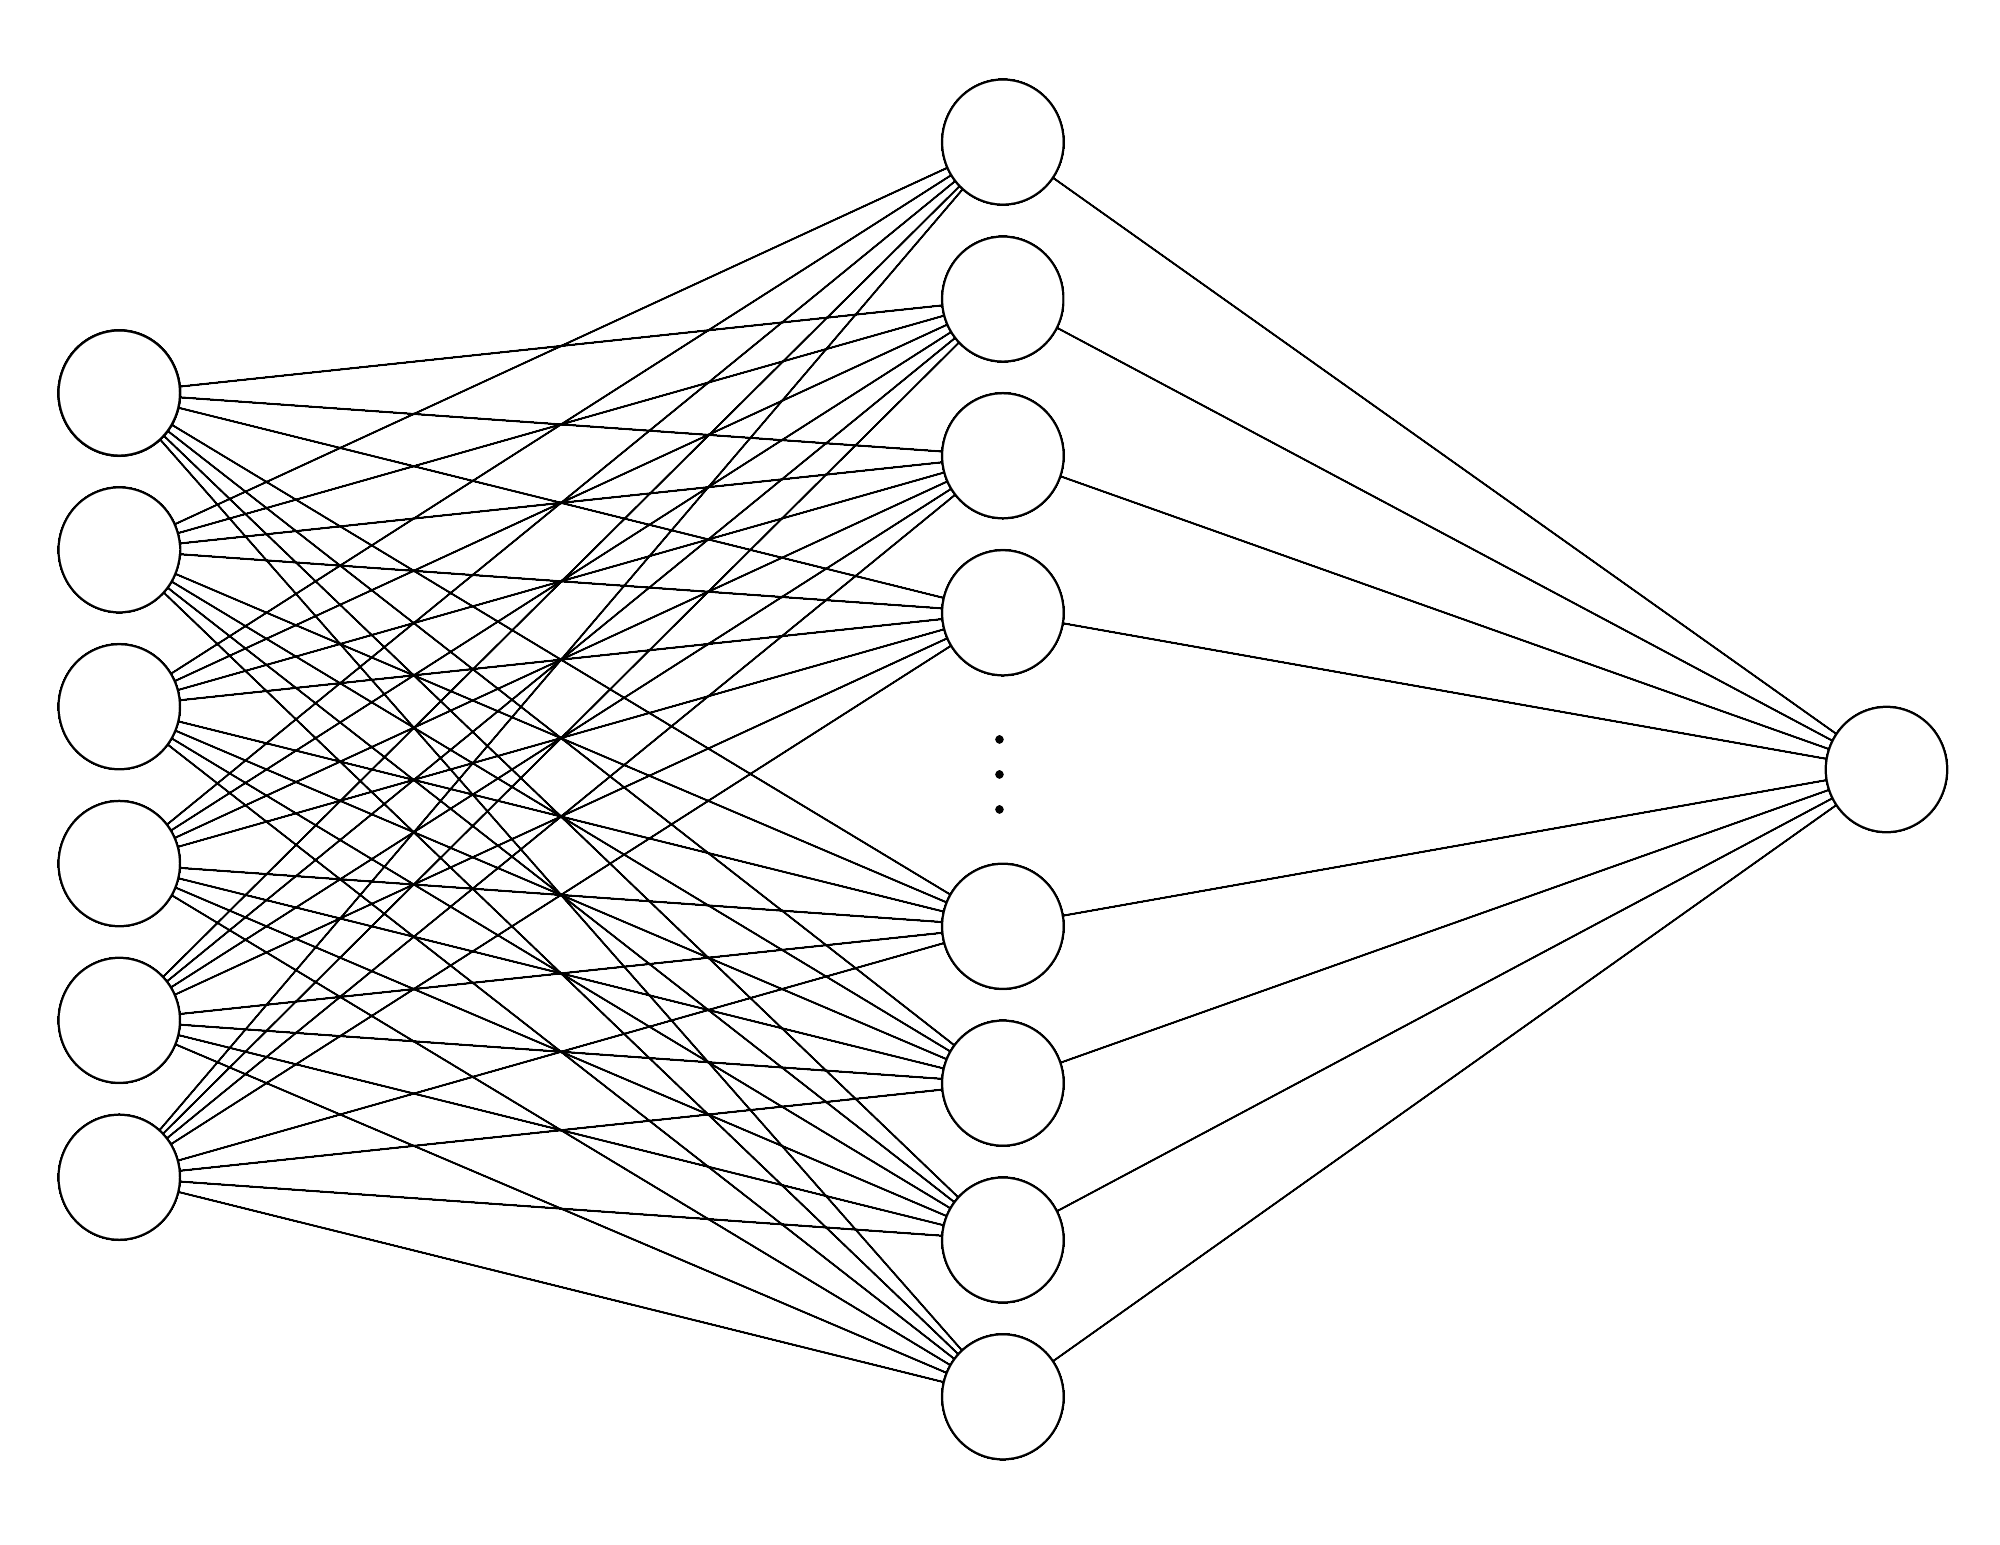
\includegraphics[width=0.8\columnwidth]{images/nn.png}
    \centering
    \caption{A fully-connected neural network with 6 nodes in the input layer, an arbitrary number of nodes in the hidden layer, and a single node in the output layer.}
    \label{fig:NN}
\end{figure}

The inputs to this neural network are the samples from two discrepant datasets with relevant cosmological parameters, and the output node is a 1D tension coordinate. Due to its popularity and effectiveness in modern deep learning applications \cite{Nwankpa2018}, a rectified linear unit (ReLU) \cite{Nair2010} is chosen as the activation function between the hidden layer and output layer.  As mentioned in Section \ref{non_gaussian}, the loss function is the Bayes Factor calculated in the 1D tension coordinate.

Training this neural network is different from training one for a classification problem. Unlike the 'traditional' method of approximating the gradient using small batches of training data \cite{Keskar2017}, we use all the data points of the two datasets to compute our gradient, and hence calculate the loss function. This method is chosen because it is crucial to provide the Bayes factor, which is our loss function, with a substantial amount of data points to better quantify the tension. We use the recently-popularised Adam optimisation algorithm \cite{Kingma2017} as our stochastic gradient descent method, with an initial learning rate of $0.001$.


\subsection{Numerical Calculation of Bayes Factor}

The calculation of the marginalised Bayes factor $R_t$ forms part of the neural network's optimisation loop. This requires the speed of the numerical computation of $R_t$ to be as rapid and efficient as possible. In this paper, we deal with datasets containing weighted samples of probability distributions in parameter space. The weighted samples of the distributions in the 1D tension coordinate is expressed as
\begin{equation}
    S_D = \big\{(t_D^{(i)}, w_D^{(i)}), i = 1, \dots , N_D \big\}, \quad t_D = T(\theta_D)
\end{equation}
where $\sum_i^{N_D} w_D^{(i)} = 1$. To numerically calculate $R_t$, we need to swap out the integral in Equation \ref{margin_R} for a sum of binned weights obtained via a histogram. 

Let us begin by defining a typical histogram as a probability density estimator. For an arbitrary weighted dataset $\{(X^{(i)}, w^{(i)}), \, i = 1, \dots , N, \, \sum_i^N w^{(i)} = 1\}$ of range $[x_0, x_1]$, bins $b^{(j)}$ and constant bin width $\Delta$, the interval of $b^{(j)}$ is defined as $[x_0 + j\Delta, x_0 + (j+1)\Delta]$. Let the centre of $b^{(j)}$ be denoted by $c^{(j)}$. The probability estimate of values in the $j$th bin is then given by
\begin{equation} \label{tophat}
    \hat{p}^{(j)}(x) = \frac{1}{\Delta} \sum_{i=1}^{N} w^{(i)} F(X^{(i)} - c^{(j)})
\end{equation}
where $x \in b^{(j)}$, and  $F$ is a top-hat function of width $\Delta$ centred at zero.

With this definition of a histogram, the marginalised Bayes factor $R_t$ can be approximated as
\begin{equation}
    R_t \approx \sum_{i}^{N_\pi} \frac{\Big(\sum_{c_A^{(j)} \in b_\pi^{(i)}} \Delta_A \hat{p}_A^{(j)}\Big) \Big(\sum_{c_B^{(j)} \in b_\pi^{(i)}} \Delta_B \hat{p}_B^{(j)}\Big)}{\Delta_\pi \hat{p}_\pi^{(i)}},
\end{equation}
where we have two datasets $A$ and $B$ with a shared prior $\pi$.

However, we have a big problem. The optimisation of the neural network uses a gradient-based method, which requires our computation of $R_t$ to be smooth and differentiable everywhere. The top-hat function $F$ in Equation \ref{tophat} is not smooth. Fortunately, we can replace $F$ with a smooth function with non-extreme derivatives to approximate a histogram. We choose a Gaussian to be the replacement of $F$ \cite{Schutt2017}, such that
\begin{equation}
    F(x) = \frac{1}{\sqrt{2\pi \sigma^2}} \exp \bigg( {-\frac{x^2}{2 \sigma^2}} \bigg)
\end{equation}
with $\sigma = \Delta / 2$. We find using such a Gaussian envelope is able to approximate a top-hat histogram quite well. [Give chi-squared?]

In practice, we find it more effective to use $\log R_t$ instead of $R_t$ as our loss function for the neural network. If we were to use $R_t$, the optimisation steps taken by the neural network becomes increasing small and ineffective as $R_t \to 0$. On the other hand, $\log R_t$ with its range of $(-\infty, \infty)$ allows gradient descent to make more confident steps towards the local minimum.

Note that instead of using a histogram as a probability density estimator, an alternative method is to use a Gaussian kernel density estimator (KDE) \cite{Silverman1986}. However, we find that the histogram method provided more stability and computational efficiency during gradient descent, hence the decision to stick with histograms using a Gaussian envelope function.



% https://stats.stackexchange.com/questions/143284/density-estimation-and-histograms

\subsection{Toy Examples}

Algorithm \ref{algo} takes us through the training of our neural network using PyTorch-esque langauge. Note that the learning rate of the optimisation method and number of epochs can be tweaked in order to reach a stable minimum of the Bayes Factor $R_t$.
\begin{algorithm}[H]
\caption{Training of Neural Network}\label{algo}
    \begin{algorithmic}[1]
    % \Procedure{Euclid}{$a,b$}\Comment{The g.c.d. of a and b}
    \State $X_A \gets $ Dataset A; $w_A \gets $ Weights A 
    \State $X_B \gets $ Dataset B; $w_B \gets $ Weights B
    \State $X_p \gets $ Prior; $w_p \gets $ Prior Weights
    \State
    \State $net \gets $ NeuralNetwork(in=6, hidden=4096, out=1)
    \State $optim \gets $ AdamOptimizer($net.parameters()$, learning\_rate=0.001)
    \State $loss \gets $ LogBayesFactor()
    \State $epochs \gets 1000$
    \State
    \For{$i \gets 0$ to $epochs$}
        \State $t_A \gets net(X_A)$ \Comment{Tension coordinates}
        \State $t_B \gets net(X_B)$
        \State $t_p \gets net(X_p)$
        \State
        \State $R_t \gets loss(t_A, t_B, t_p, w_A, w_B, w_p)$
        \State $R_t.backward()$ \Comment{Compute gradients of neural network parameters}
        \State $optim.step()$ \Comment{Make gradient descent step}
    \EndFor
    \State
    \State \textbf{return} $net$
    \end{algorithmic}
\end{algorithm}

Before applying the neural network onto cosmological datasets, we first verify our method using toy datasets. We generate 10000 samples from each of the distributions described below to create our toy datasets.

The very simplest case to begin with would be two disagreeing 2D Gaussian distributions. In our example, we place these two distributions around $5\sigma$ apart, and encase them in an arbitrary square prior, as seen in Figure \ref{fig:toy}(a). Our neural network is able to fit rough hyperplanes perpendicular to a line connecting the two distributions. This is a result that agrees with the analytical tension coordinate for the Gaussian case derived in Section \ref{gaussian_tension}. Our neural network is working so far.

The next example can be seen in Figure \ref{fig:toy}(b). We are still working in two dimensions, but now we have a Gaussian distribution accompanied by a concave quarter-circle distribution. Again, we have a square prior. With this setup, we expect the hypersurfaces, or more simply the contour lines, to be shaped around the 'banana-like' distribution, with directions of maximum tension radiating outwards from the central Gaussian distribution. This is exactly what we see from our results, as illustrated in Figure \ref{fig:toy}(b). It is important to note that the statistical power of our neural network only lies in the region between and close to our two distributions, and starts to falter as we navigate further away. This effect can be noticed at the ends of the 'banana', where we see the contour lines beginning to bend away from the curve of the distribution. Our neural network is working well.

\begin{figure}
    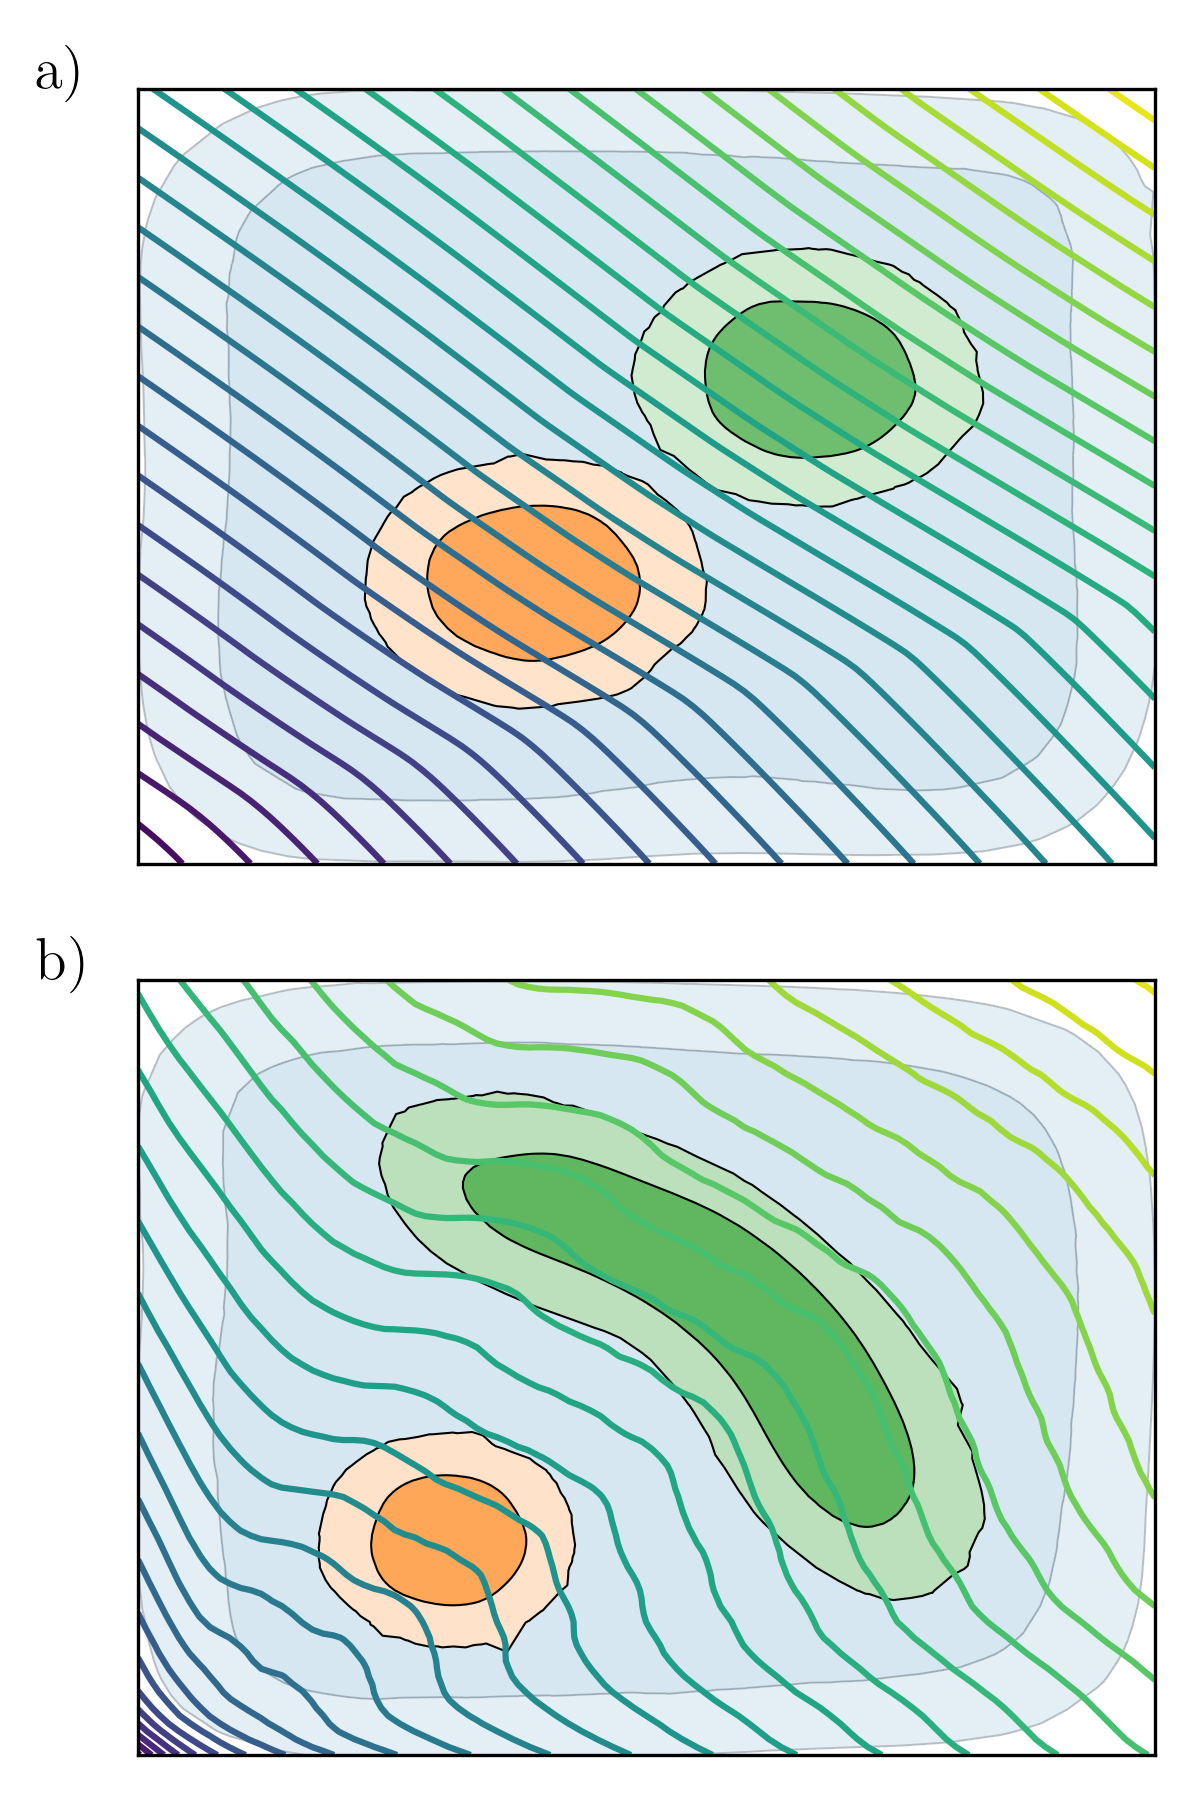
\includegraphics[width=0.8\columnwidth]{../plots/toy.png}
    \centering
    \caption{These contour plots illustrate the hypersurfaces shaped by the neural network after training for 500 epochs. a) shows two Gaussian distributions and b) shows a Gaussian distribution accompanied by a 'banana-shaped' distribution. The faded blue distribution in the background is the prior.}
    \label{fig:toy}
\end{figure}


\subsection{Cosmological Dataset}

In this paper, we work solely with cosmological measurements made by the DES and the \textit{Planck} satellite. We choose these two datasets because of the well reported tensions between them in recent years \cite{Handley2019, Lemos2020}. The tensions mentioned in Section \ref{intro} of this paper, such as the $3\sigma$ tension in the $\Omega_m$ and $\sigma_8$ plane, also do exist between these two datasets.

We use the following six cosmological parameters -- physical baryon density $\Omega_b h^2$, matter density $\Omega_m$, Hubble constant $H_0$, optical depth to reionisation $\tau$, matter fluctuation amplitude $\sigma_8$, and scalar power law index $n_s$. The derived parameters of $\Omega_m$, $H_0$ and $\sigma_8$ are chosen over three other independent cosmological parameters because tensions in these parameters are well-known. Applying our neural network to these parameters with well-established discrepancies allows us to verify and reinforce the existing tension in them.

We obtain the DES Y1 and \textit{Planck} datasets from \cite{Dataset}. This source provides nested sampling chains for all of the relevant independent, derived and nuisance parameters of both datasets. We use the \texttt{anesthetic} Python library \cite{anesthetic} to extract weighted samples from the nested sampling chains.


\subsection{Identifying Source(s) of Tension}


\section{Results and Discussion}

\section{Conclusions}





\begin{acknowledgments}

\end{acknowledgments}

\appendix

\section{Appendixes}

\section{A little more on appendixes}


\subsection{\label{app:subsec}A subsection in an appendix}




% The \nocite command causes all entries in a bibliography to be printed out
% whether or not they are actually referenced in the text. This is appropriate
% for the sample file to show the different styles of references, but authors
% most likely will not want to use it.

\bibliography{apssamp}% Produces the bibliography via BibTeX.

\end{document}
%
% ****** End of file apssamp.tex ******